\documentclass[11pt]{article}
\usepackage[margin=1in]{geometry}
\usepackage{graphicx}
\usepackage{booktabs}
\usepackage{hyperref}
\usepackage{siunitx}
\usepackage{float}
\usepackage{caption}
\usepackage{subcaption}
\usepackage{enumitem}

\title{Checkpoint 1: Exploratory Data Analysis\\CPSC 4300/6300 Applied Data Science}
\author{Michael Joseph Ellis}
\date{\today}

\begin{document}
\maketitle

\section*{Background, Objective, and Framing}
The dataset \emph{Students Performance Dataset} provides records for 2{,}392 synthetic high-school students with demographics, study habits, parental involvement, extracurricular activities, and academic outcomes. Our objective for the semester project is to build a predictive model that estimates a student's final grade category, \texttt{GradeClass}, using the provided features. This frames the problem as a supervised multi-class classification task. We will ultimately evaluate tree-based gradient boosting models (e.g., XGBoost) and compare against strong baselines.

\paragraph{Rationale.} \texttt{GradeClass} is an ordinal categorical outcome derived from GPA. Predicting \texttt{GradeClass} is useful in practice (early warning and support targeting) and aligns with the project's emphasis on interpretable, actionable features (study time, absences, parental support, etc.).

\section*{Dataset Summary}
	\textbf{Source and unit of analysis.} Data are downloaded from Kaggle (Rabie El Kharoua, CC BY 4.0). Each row corresponds to a unique student (\texttt{StudentID}). The file used is \texttt{Student\_performance\_data \_.csv}. The class labels are coded as: 0=A, 1=B, 2=C, 3=D, 4=F.

	\textbf{Size.} The dataset contains 2{,}392 observations (all unique) and 15 columns (including the target). All students are ages 15--18.

	\textbf{Key variables.} Demographics (Age, Gender, Ethnicity, ParentalEducation), study habits (StudyTimeWeekly, Absences, Tutoring), parental involvement (ParentalSupport), extracurriculars (Extracurricular, Sports, Music, Volunteering), performance (GPA), and target (GradeClass).
\begin{figure}[H]
	\centering
	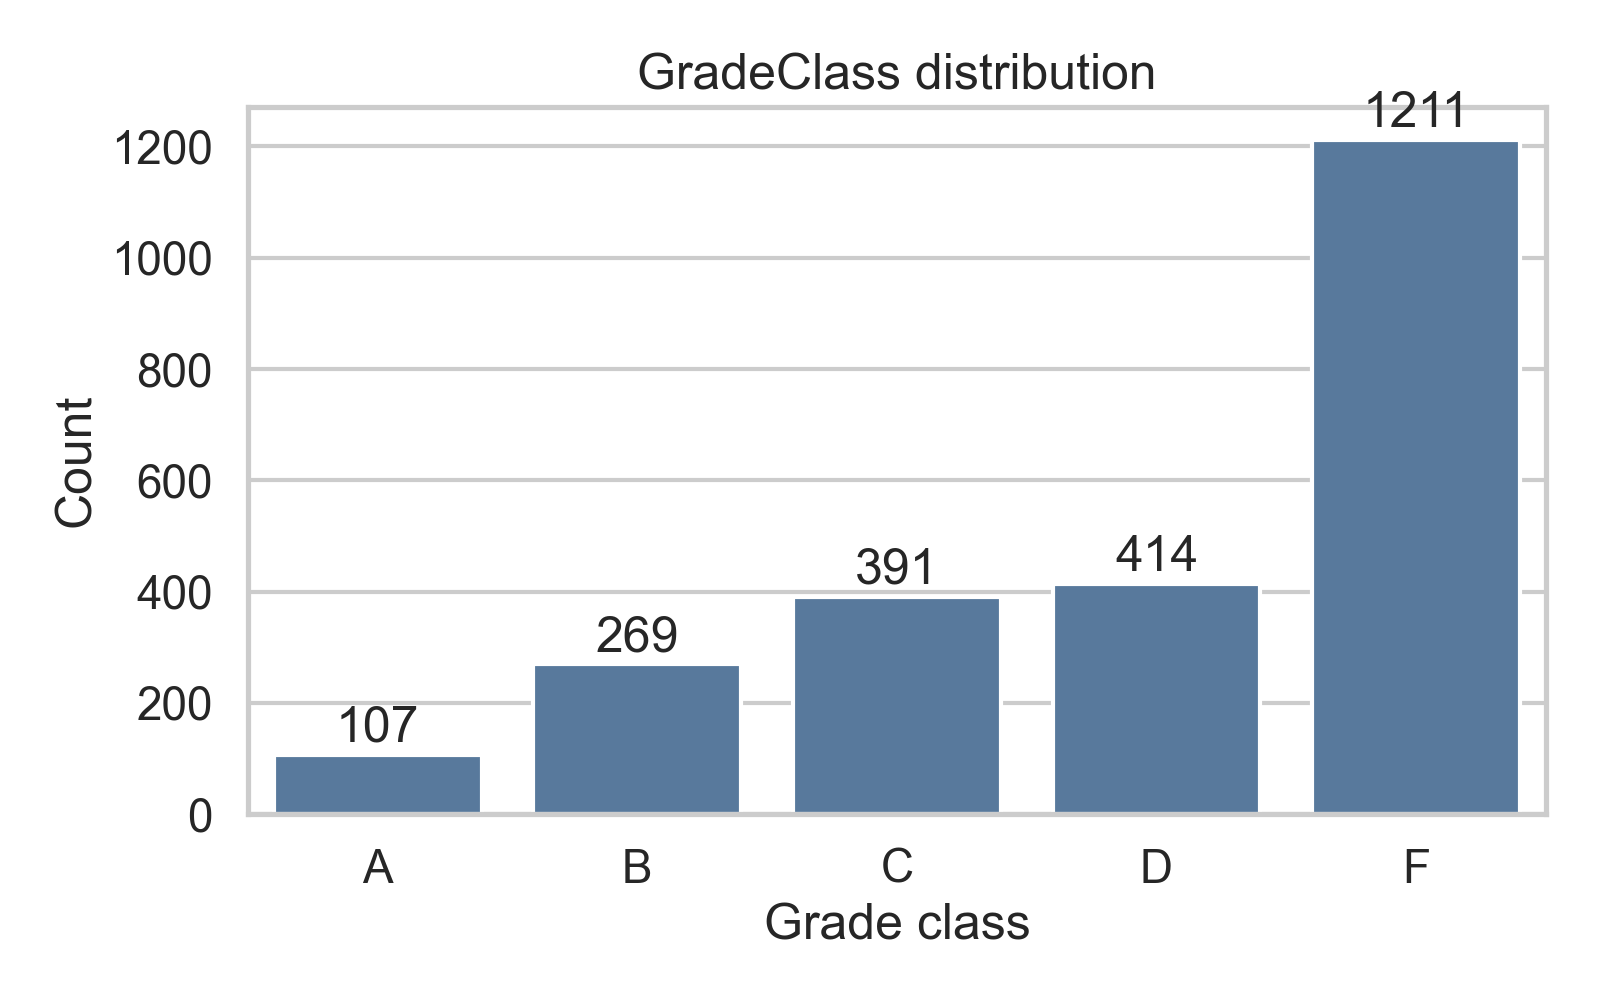
\includegraphics[width=.6\textwidth]{figures/gradeclass_distribution.png}
	\caption{Distribution of GradeClass (A--F).}\label{fig:gradeclass-dist}
\end{figure}

\begin{figure}[H]
	\centering
	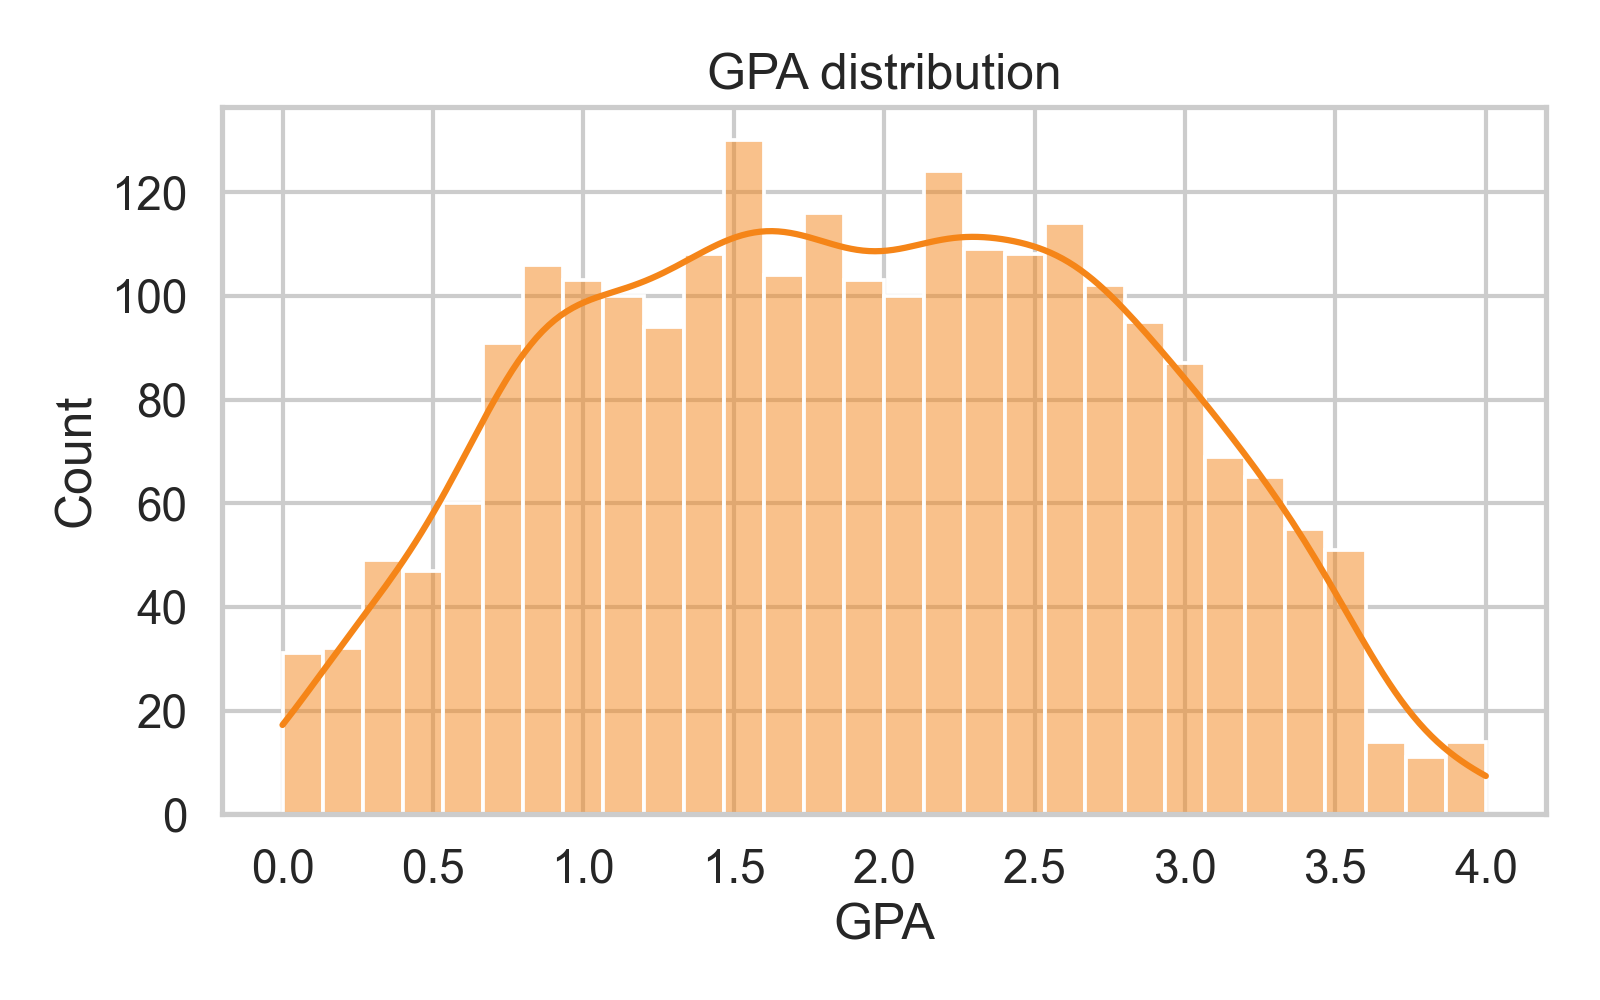
\includegraphics[width=.65\textwidth]{figures/gpa_histogram.png}
	\caption{GPA distribution.}\label{fig:gpa-hist}
\end{figure}

\section*{Data Cleaning Summary}
We verified that \texttt{StudentID} is unique (2{,}392 unique IDs for 2{,}392 rows) and computed per-column missingness. The exported audit file (\texttt{figures/missingness.csv}) shows \emph{zero} missing values across all columns, so no rows were dropped and no imputations were applied. Basic range checks matched the data card: Age 15--18; StudyTimeWeekly 0--20 hours; Absences 0--30; and GPA 0--4. Categorical fields (e.g., Gender, Ethnicity, ParentalEducation, Tutoring, ParentalSupport, Extracurricular, Sports, Music, Volunteering) are currently integer-coded and were left as-is for EDA; for modeling we will treat them as categorical (e.g., one-hot encoding).

We did not remove potential outliers at this stage. Distributions show expected tails (e.g., higher absences and lower GPA for some students) that are plausible for the domain. Tree-based boosting methods are robust to such values; we will revisit outlier influence during model diagnostics.

\section*{Outcome Variable}
	\textbf{Definition.} \texttt{GradeClass} is derived from GPA with bins: A ($\geq 3.5$), B ($[3.0,3.5)$), C ($[2.5,3.0)$), D ($[2.0,2.5)$), and F ($<2.0$). We visualize the distribution above and the underlying GPA shape to understand separability across bins.

\section*{Initial Feature Exploration}
We inspected several hypothesized drivers of performance.

\begin{figure}[H]
	\centering
	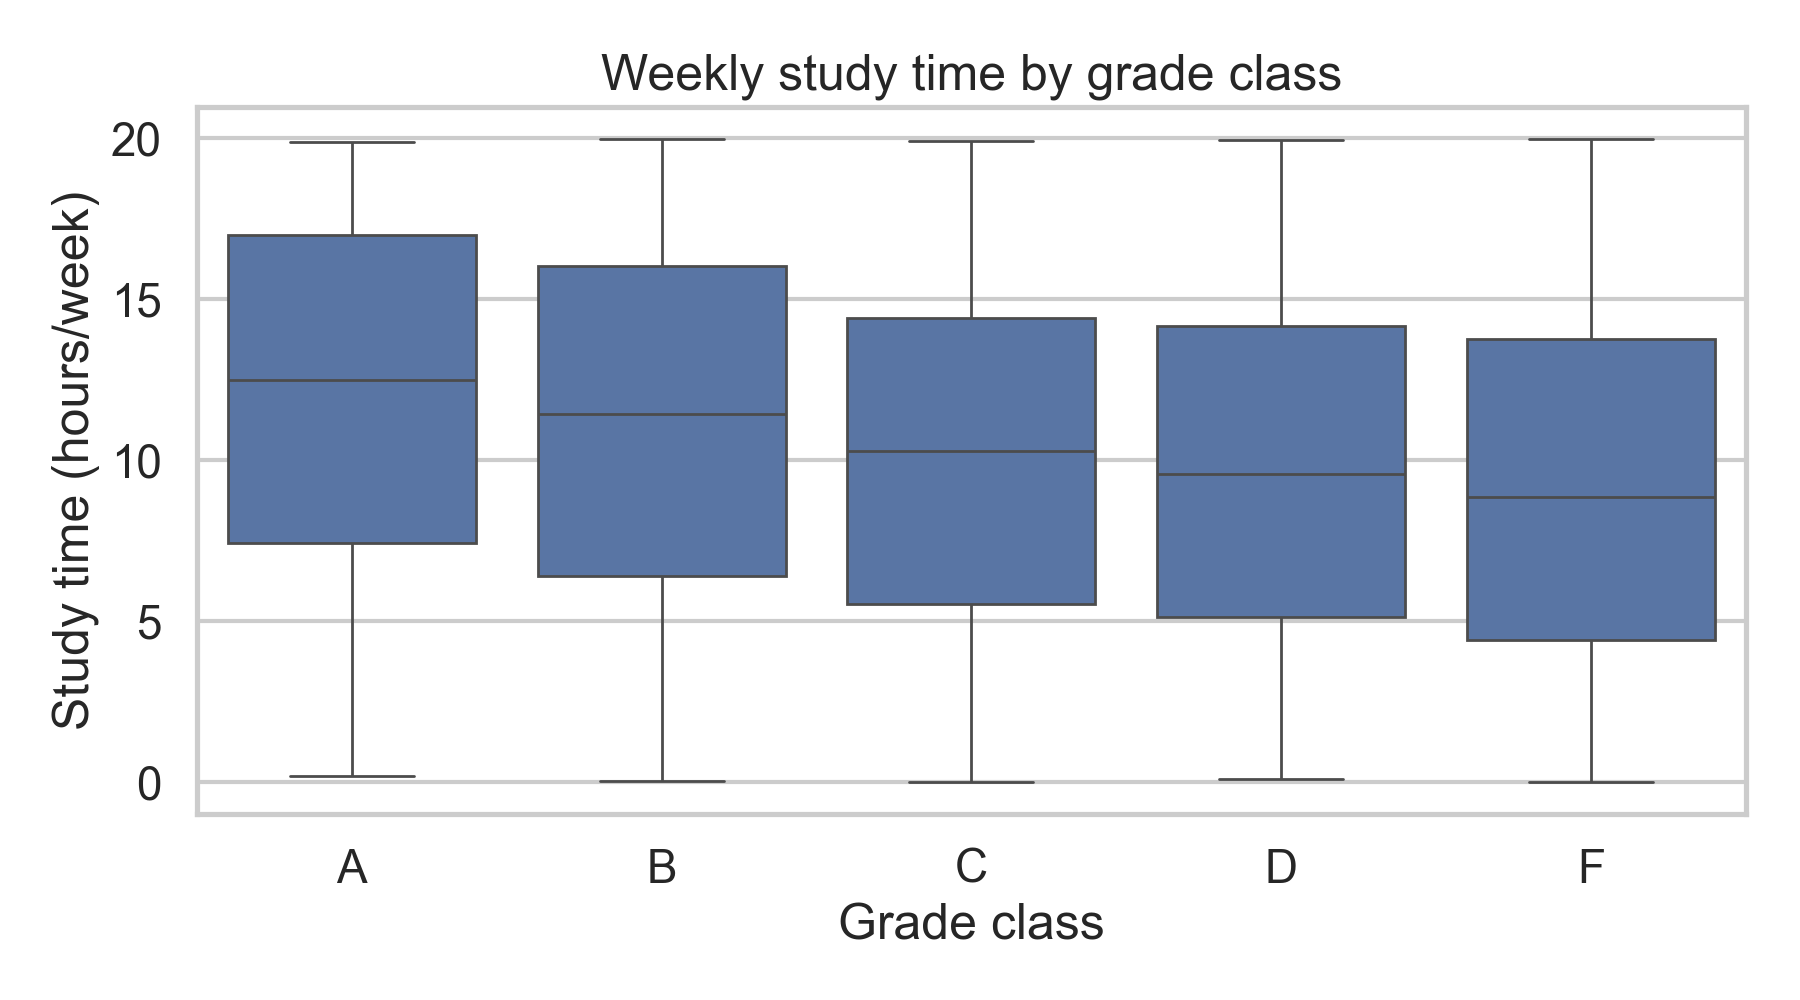
\includegraphics[width=.9\textwidth]{figures/studytime_by_gradeclass.png}
	\caption{Weekly study time vs. grade class. Higher study time is associated with stronger letter grades.}\label{fig:studytime}
\end{figure}

\begin{figure}[H]
	\centering
	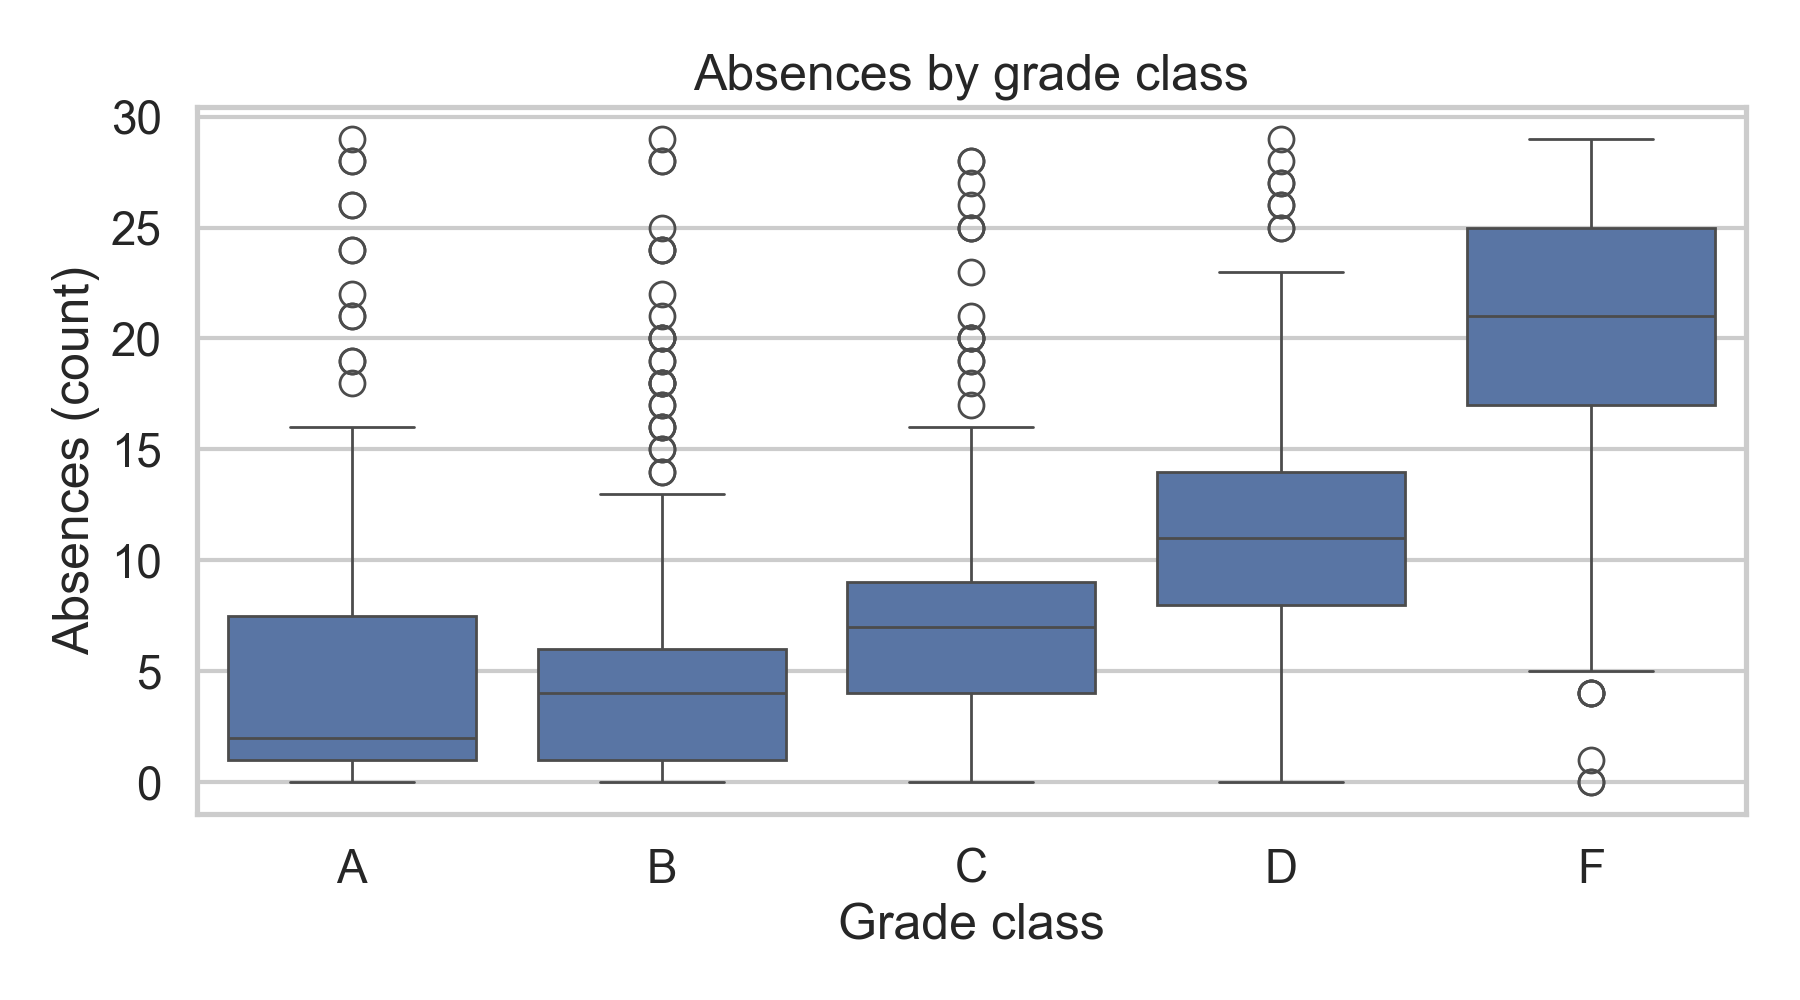
\includegraphics[width=.9\textwidth]{figures/absences_by_gradeclass.png}
	\caption{Absences vs. grade class. More absences correlate with lower grades.}\label{fig:absences}
\end{figure}

\begin{figure}[H]
	\centering
	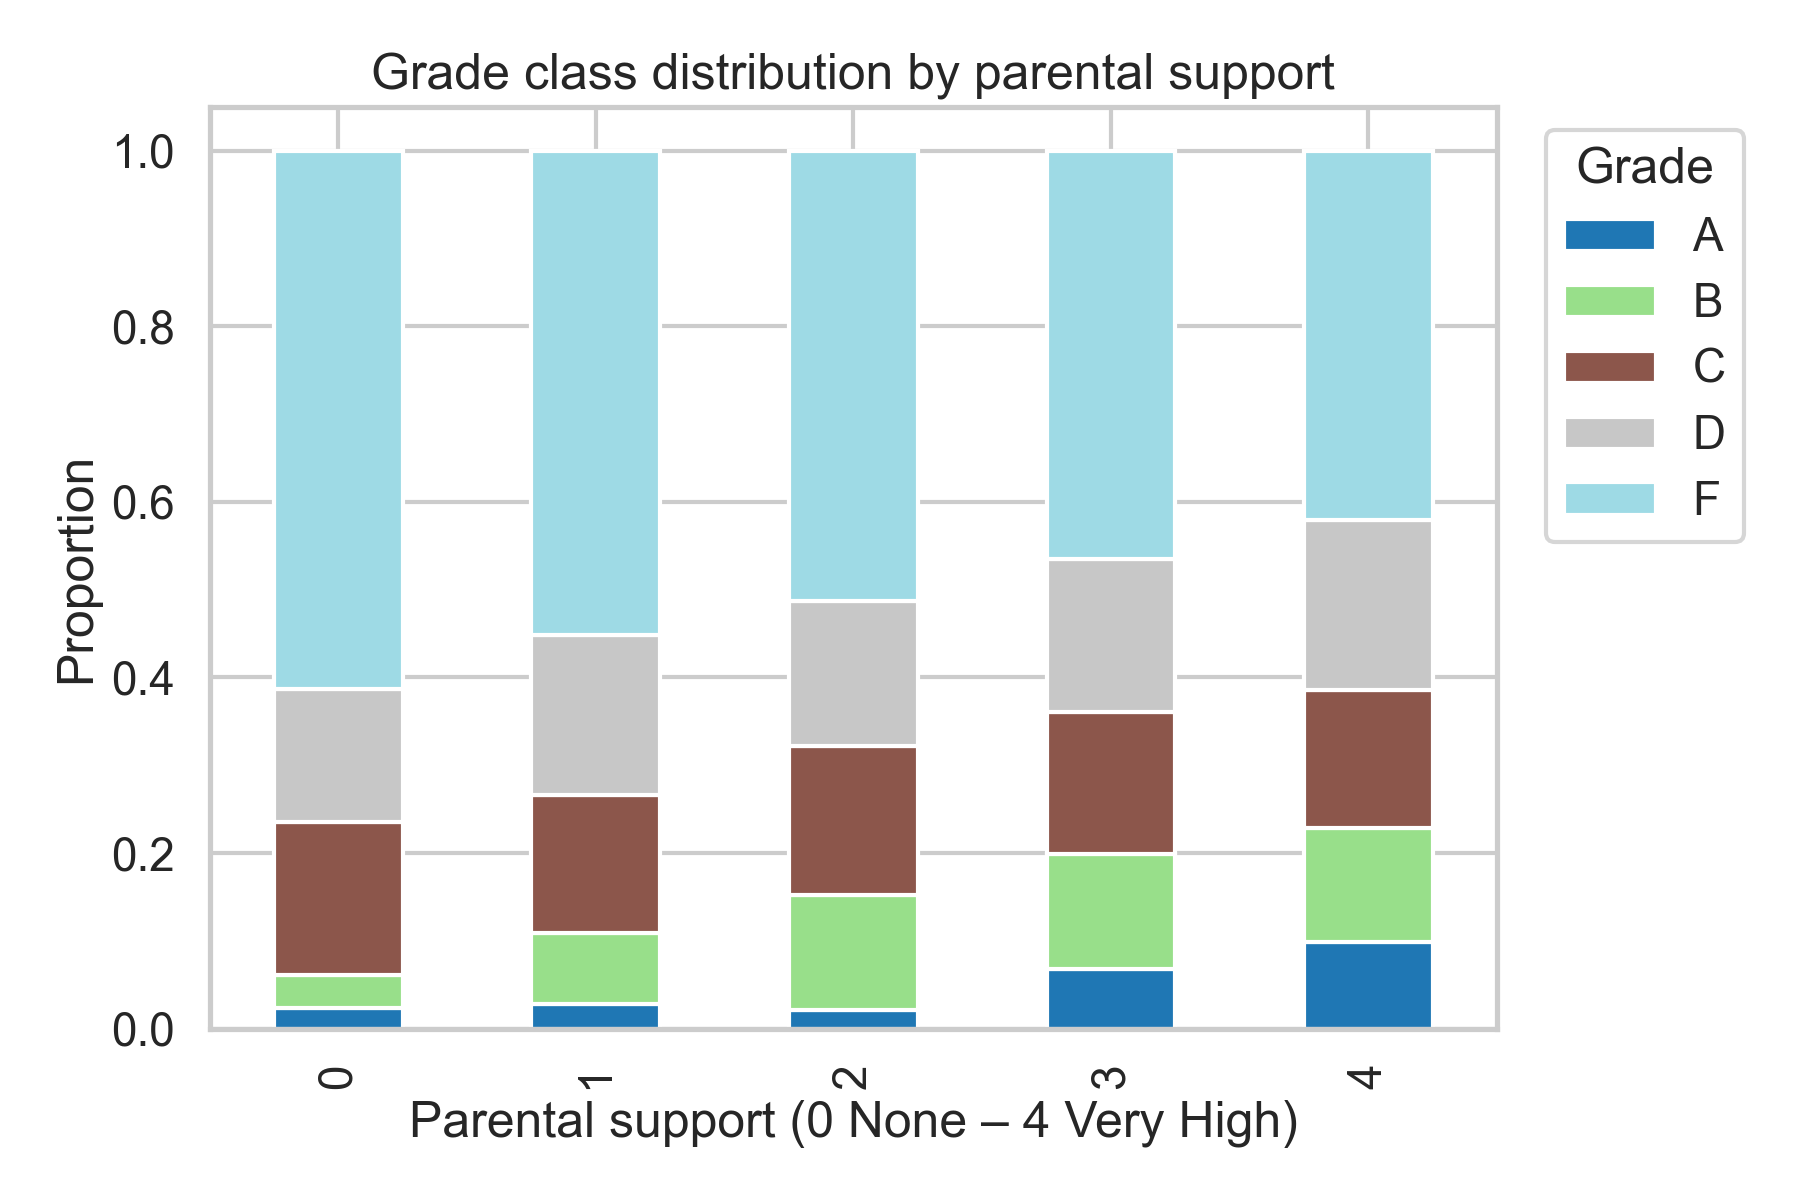
\includegraphics[width=.9\textwidth]{figures/parental_support_vs_gradeclass.png}
	\caption{Grade-class composition by parental support level. Greater support shifts mass toward A/B.}\label{fig:parental-support}
\end{figure}

\begin{figure}[H]
	\centering
	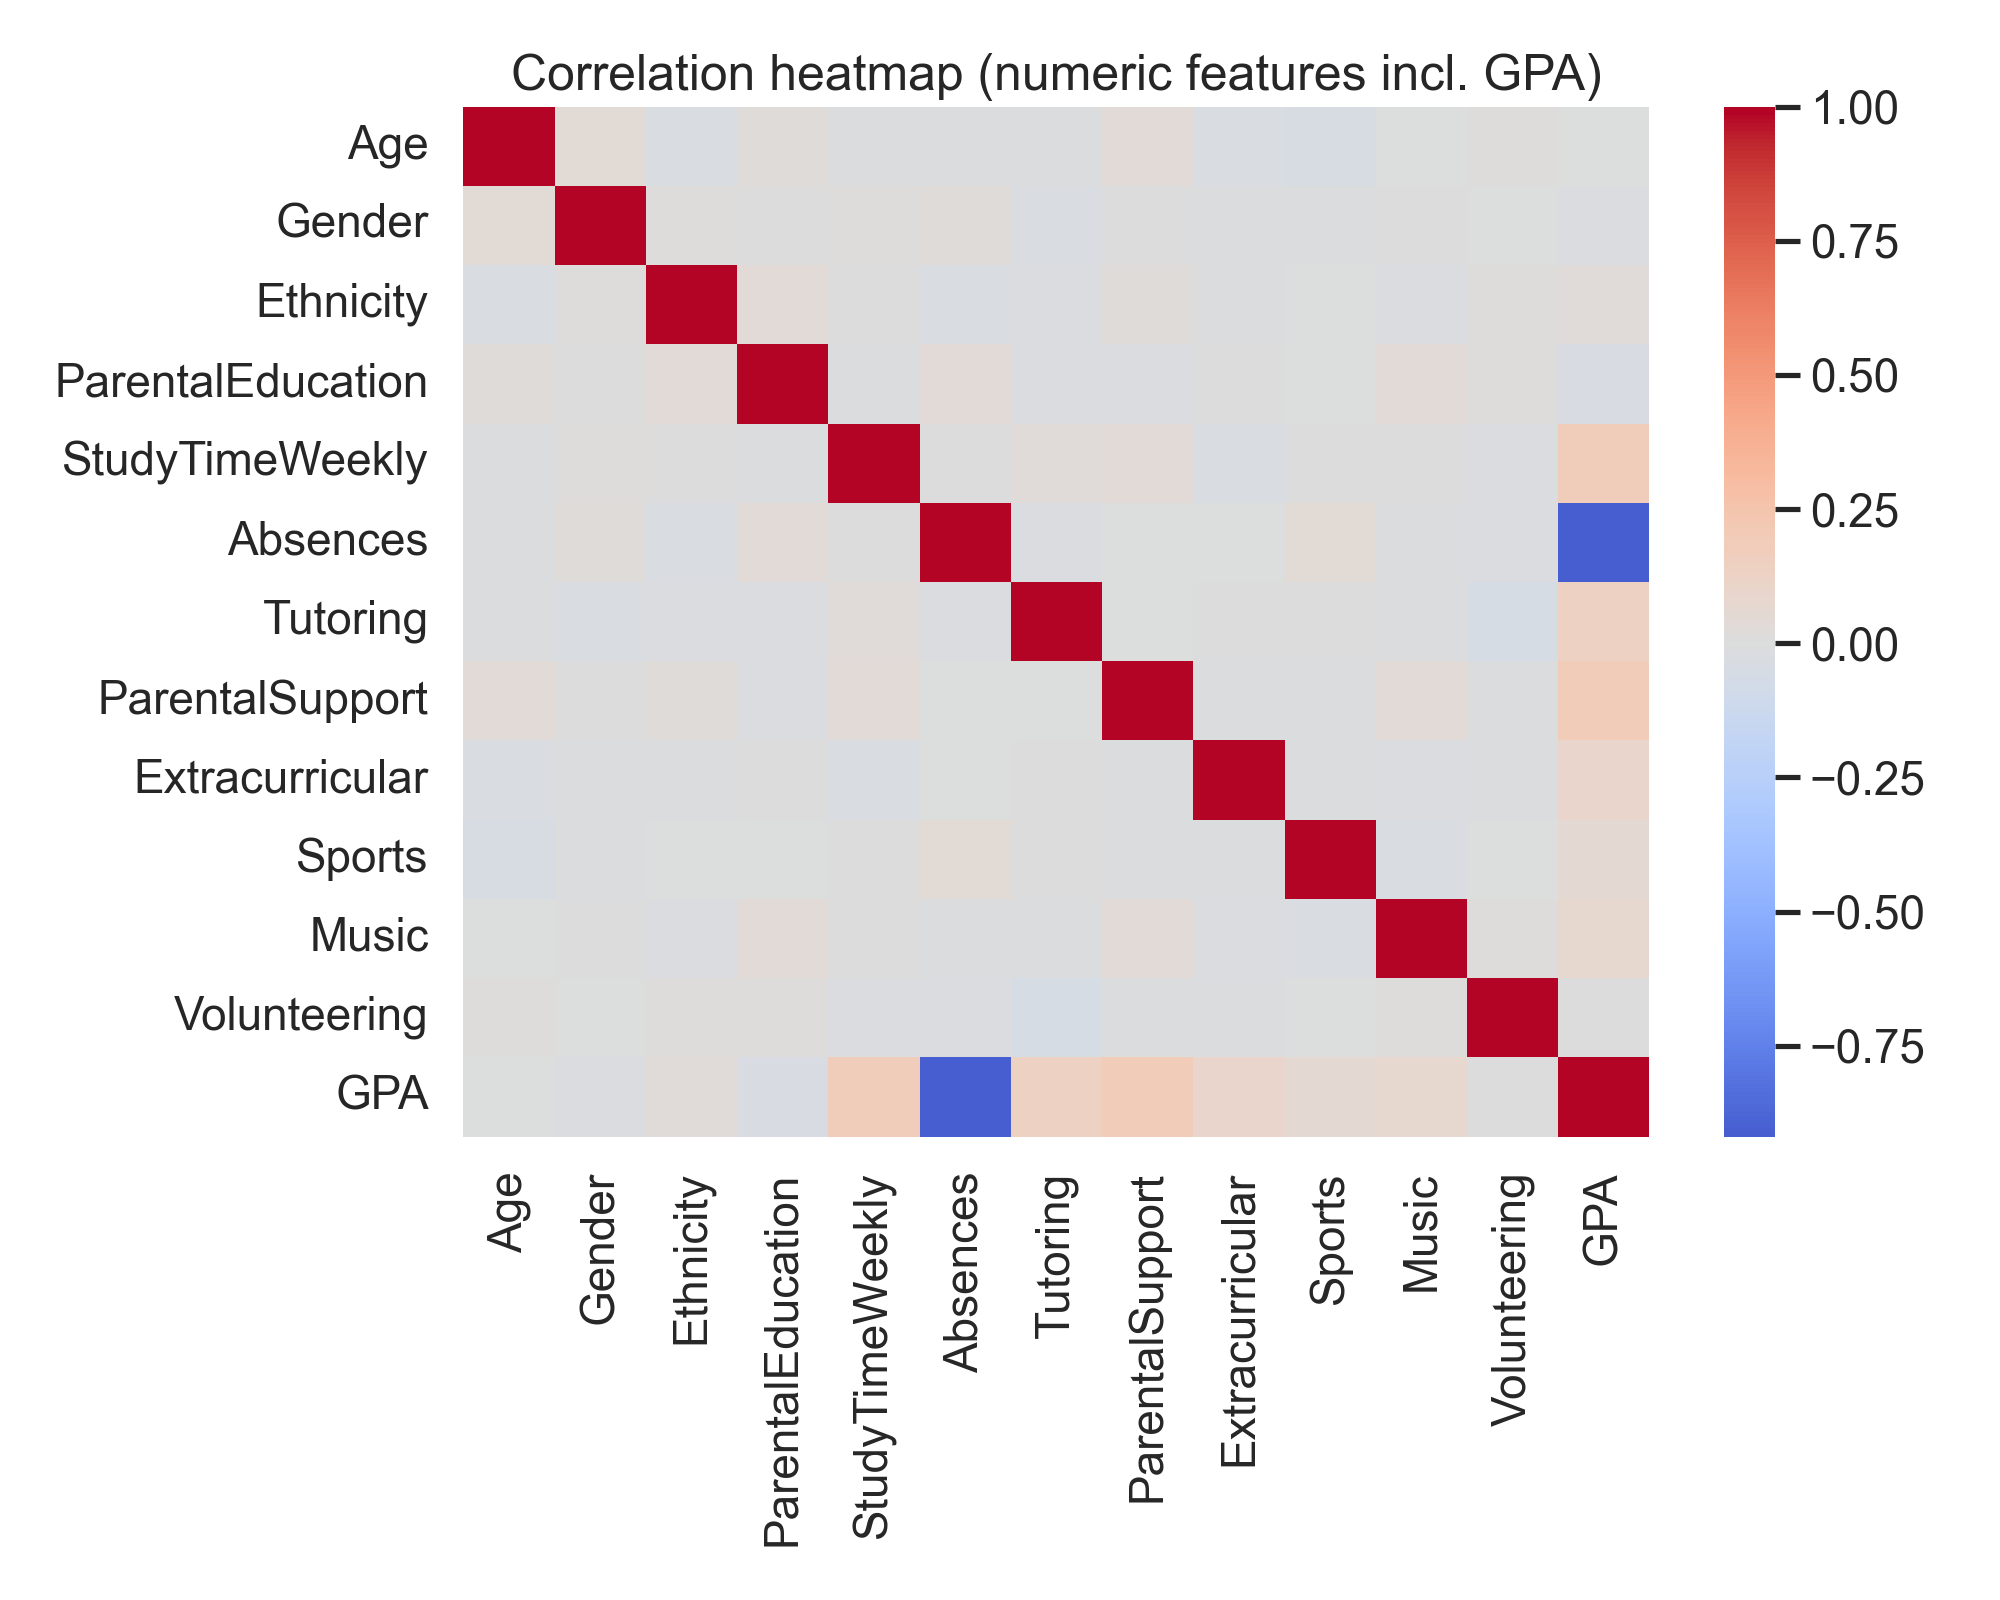
\includegraphics[width=.9\textwidth]{figures/correlation_heatmap.png}
	\caption{Correlation heatmap among numeric variables (including GPA).}\label{fig:corr-heatmap}
\end{figure}

\section*{Key Predictors for Modeling}
We compared each candidate predictor to the response using distribution plots and simple summaries. Three features consistently showed the clearest relationships with performance:
\begin{itemize}[leftmargin=*]
	\item \textbf{Absences}: Strong negative association with performance. Spearman correlation with GPA is $\approx -0.93$. Median absences rise monotonically across grade bins: A=2, B=4, C=7, D=11, F=21. The boxplot in Figure~\ref{fig:absences} shows a sharp shift toward higher absence counts for lower grades.
	\item \textbf{StudyTimeWeekly}: Positive association with performance. Spearman with GPA is $\approx 0.17$. Median weekly study time decreases from A ($\approx 12.5$ h/wk) to F ($\approx 8.8$ h/wk). While the effect is weaker than absences, it is consistent and practically interpretable for interventions.
	\item \textbf{ParentalSupport}: Positive association with performance. Spearman with GPA is $\approx 0.18$. The share of A/B among students with high support (levels 3--4) is about 20.7\%, compared to 9.4\% among those with low support (levels 0--1), reflecting a meaningful shift in grade mix (see stacked bars).
\end{itemize}

\noindent\textbf{Selection for this assignment.} In line with the rubric (choose one or two predictors), we select \textbf{Absences} and \textbf{StudyTimeWeekly} as the most important initial predictors:
\begin{enumerate}[leftmargin=*]
	\item \emph{Absences} has the strongest empirical signal and a clear causal story (missed classes reduce learning opportunity).
	\item \emph{StudyTimeWeekly} is actionable (students can adjust effort) and complements Absences by capturing productive engagement outside class.
\end{enumerate}
ParentalSupport will be included in subsequent modeling as an additional contextual predictor but we prioritize the two above for Checkpoint 1.

\section*{Modeling Plan (Preview)}
For Checkpoint 2, we will implement an XGBoost multi-class classifier (softmax objective) with a stratified train/validation split and macro-averaged F1 as the primary metric. Categorical features coded as integers will be treated as ordered or one-hot encoded as appropriate; we will compare both encodings. We will include simple preprocessing (imputation and scaling where needed) inside a scikit-learn pipeline to keep evaluation clean and reproducible.

\section*{Reproducibility}
All figures in this report are generated by \texttt{data analysis/reader.py} and saved to \texttt{Checkpoint 1/figures/}. Dependencies are listed in \texttt{requirements.txt}.

\noindent The complete code, CSV, and rendered figures are available in the public repository:
\begin{itemize}[leftmargin=*]
	\item GitHub (this project path): \url{https://github.com/Michael-Joseph-Ellis/disgusting-undergrad-busy-work/tree/main/CPSC%20Coursework/CPSC4300/Semester-Project}
	\item Data analysis code (modular): \texttt{CPSC Coursework/CPSC4300/Semester-Project/data analysis/eda/} (\texttt{main.py}, \texttt{plots.py}, \texttt{loader.py}, \texttt{stats.py}, \texttt{paths.py}); 
	\item Figures generated by EDA: \texttt{CPSC Coursework/CPSC4300/Semester-Project/Checkpoint 1/figures/}
\end{itemize}

\vspace{.5em}
\noindent\textbf{License/Citation.} Dataset: Rabie El Kharoua, ``Students Performance Dataset'', CC BY 4.0, retrieved from \url{https://www.kaggle.com/datasets/rabieelkharoua/students-performance-dataset}.

\end{document}